%%%%%%%%%%%%%%%%%%%%%%%%%%%%%%%%%%%%%%%%%%%%%%%%%%%%%%%%%%
%
% Doctoral Thesis Template @ The University of Manchester
% LaTeX Chapter Template
% Version 1 (23/07/2020)
% Joe Crone
%
% This template is based on:
% The University of Manchester, Presentation of Thesis Policy
% Research Office Graduate Education Team
% June 2017
% http://www.regulations.manchester.ac.uk/pgr-presentation-theses/
%
%%%%%%%%%%%%%%%%%%%%%%%%%%%%%%%%%%%%%%%%%%%%%%%%%%%%%%%%%%
\documentclass[../main.tex]{subfiles}
\begin{document}

% Title
%--------------------------------------------------------
\chapter{Theory of Photon Production by Inverse Compton Scattering}
\label{Theory_of_Photon_Production_by_Inverse_Compton_Scattering} % to reference use \ref{ChapterTemplate}

\begin{equation}
\frac{\omega'}{\omega} = \gamma\left(1+\beta\cos\theta\right),
\label{eq:doppler_shift}
\end{equation}
where $\omega'$ is the Doppler shifted angular frequency, $\omega$ is the incident photon angular frequency, $\beta$ is the Lorentz speed factor and $\theta$ is the angle between the incident and Doppler shifted photon. 

\textcolor{blue}{**TALK ABOUT THE REGIMES OF INVERSE COMPTON SCATTERING, NON-LINEAR AND RECOIL**}

\begin{figure}[!htb]
    \centering
    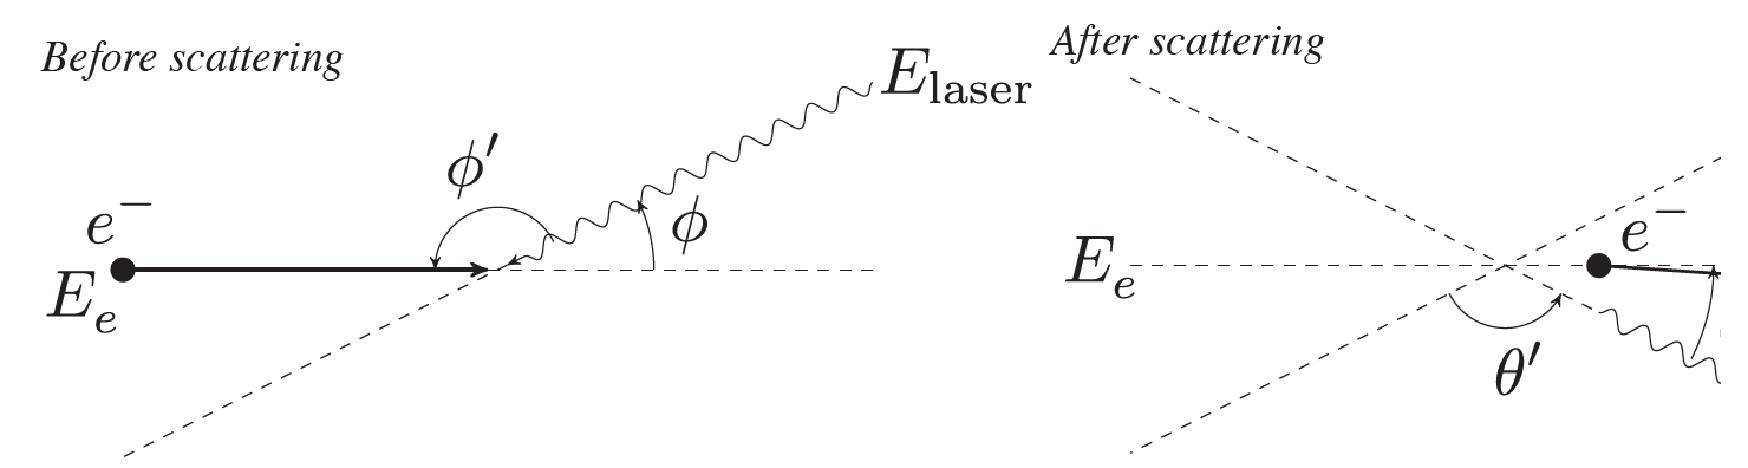
\includegraphics[width=\textwidth]{Figures/Theory_of_Photon_Production_by_Inverse_Compton_Scattering/scatteringkinematicsdiagram.pdf}
    \caption{Geometry of the inverse Compton scattering event at the interaction point. This geometry follows the geometry prescribed by Sun et al \cite{sun2009energy}. }
    \label{fig:scattered_photon_kinematics}
\end{figure}

\textcolor{blue}{**DERIVATION OF THE ICS SCATTERED PHOTON ENERGY**\\}

Motivated by the geometry of the inverse Compton scattering process as shown in Figure \ref{fig:scattered_photon_kinematics}, we can write the initial photon $Q_{i}$ and electron $P_{i}$ four-vectors

\begin{align}
Q_{i} = \frac{E_{L}}{c}\left(1,\hat{n}_{i}\right), \\
P_{i} = \gamma m\left(c,\boldsymbol{v_{i}}\right),
\label{eq:initial_four_vectors}
\end{align}
where $E_{L}$ is the energy of the incident photon, $\hat{n}_{i}$ is the unit displacement three-vector of the incident photon, $\gamma$ is the Lorentz factor, $m$ is the mass of the electron, $c$ the speed of light in a vacuum and $\boldsymbol{v_{i}}$ is the velocity three-vector of the incident electron with magnitude $v_{i}$. Similarly, we can present the final electron and scattered photon states with the four-vectors 

\begin{align}
Q_{f} = \frac{E_{\gamma}}{c}\left(1,\hat{n}_{f}\right),
P_{f} = \gamma' m\left(c,\boldsymbol{v_{f}}\right),
\label{eq:final_four_vectors}
\end{align}

where $E_{\gamma}$ is the scattered photon energy, $\hat{n}_{f}$ is the unit displacement three-vector of the scattered photon, $\gamma'$ is the Lorentz factor of the recoiling electron and $\boldsymbol{v_{f}}$ is the velocity three-vector of the recoiling electron with magnitude $v_{f}$. At this point we can consider our Lorentz invariant quantities 

\begin{align}
P_{\mu}P^{\mu} = \gamma^{2}m^{2}\left(v^{2}-c^{2}\right) = -m^{2}c^{2},
\label{eq:lorentz_invariants1} \\
Q_{\mu}Q^{\mu} = 0.
\label{eq:lorentz_invariants2}
\end{align}

In the inverse Compton scattering the conservation of four-momentum can be wrote as

\begin{equation}
P_{i} + Q_{i} = P_{f} + Q_{f}.
\label{eq:conservation_four_momentum}
\end{equation}

We can multiply Eq. \ref{eq:conservation_four_momentum} by the final four momentum of the scattered photon and apply Eq. \ref{eq:lorentz_invariants2} the Lorentz invariant 

\begin{align}
Q_{f}^{\mu}\left(P_{i\mu} + Q_{i\mu}\right) = Q_{f}^{\mu}\left(P_{f\mu} + Q_{f\mu}\right), \\
Q_{f}^{\mu}P_{i\mu}+Q_{f}^{\mu}Q_{i\mu} = Q_{f}^{\mu}P_{f\mu}.
\label{eq:apply_photon_pfinal}
\end{align}
 
Similarly we can construct another equation by inspecting the square of the conservation of four-momentum

\begin{align}
\left(P_{i}+Q_{i}\right)_{\mu}\left(P_{i}+Q_{i}\right)^{\mu} = \left(P_{f}+Q_{f}\right)_{\mu}\left(P_{f}+Q_{f}\right)^{\mu}, \\
P_{i\mu}P_{i}^{\mu}+Q_{i\mu}P_{i}^{\mu}+Q_{i\mu}P_{i}^{\mu}+Q_{i\mu}Q_{i}^{\mu} = P_{f\mu}P_{f}^{\mu}+Q_{f\mu}P_{f}^{\mu}+P_{f\mu}Q_{f}^{\mu}+Q_{f\mu}Q_{f}^{\mu},
\label{eq:apply_conservation_squared}
\end{align}
utilising the commutation of four-vectors ($P_{\mu}Q^{\mu} = Q_{\mu}P^{\mu}$) and our Lorentz invariants Eq. \ref{eq:lorentz_invariants1}, \ref{eq:lorentz_invariants2} we can simplify this further

\begin{equation}
P_{i\mu}Q_{i}^{\mu} = P_{f\mu}Q_{f}^{\mu}.
\label{eq:end_conservation_squared}
\end{equation}
Subbing Eq. \ref{eq:end_conservation_squared} into Eq. \ref{eq:apply_photon_pfinal} yields

\begin{equation}
Q_{f}^{\mu}P_{i\mu}+Q_{f}^{\mu}Q_{i\mu} = Q_{i}^{\mu}P_{i\mu}
\label{eq:substitution_four_vector}
\end{equation}

Which in three-vector notation is shown as

\begin{equation}
\frac{E_{L}E_{\gamma}}{c^{2}}\left(\hat{n}_{i}\cdot\hat{n}_{f}-1\right)+\frac{E_{\gamma}}{c}\gamma m\left(\hat{n}_{f}\cdot \boldsymbol{v_{i}}-c\right) = \frac{E_{L}}{c}\gamma m\left(\hat{n}_{i}\cdot \boldsymbol{v_{i}} -c\right)
\label{eq:three_vector_solution}
\end{equation}

However, Eq. \ref{eq:three_vector_solution} should be presented in terms of the angles in Figure \ref{fig:scattered_photon_kinematics}. The dot products within this formula can be replaced using projections to introduce the angular dependencies

\begin{align}
\hat{n}_{i}\cdot\hat{n}_{f} = \cos\theta',
\label{eq:projection_angle_incident_scattered_photon}\\
\hat{n}_{f}\cdot \boldsymbol{v_{i}} = v_{i}\cos\theta,
\label{eq:projection_scattering_angle}\\
\hat{n}_{i}\cdot \boldsymbol{v_{i}} = v_{i}\cos\phi'.
\label{eq:projection_pi_minus_crossing_angle}
\end{align}
where $\phi'=\pi-\phi$ with $\phi$, the crossing angle, which is the angle between the incident photon and the incident electron, $\theta$ is the angle between the incident electrons and the scattered photons and $\theta'=\phi'-\theta$ is the angle between the incident and scattered photons. Upon subbing in the projections (Eq. \ref{eq:projection_angle_incident_scattered_photon}, \ref{eq:projection_scattering_angle}, \ref{eq:projection_pi_minus_crossing_angle}) Eq. \ref{eq:three_vector_solution} becomes

\begin{equation}
E_{L}E_{\gamma}\left(\cos\theta'-1\right)+E_{\gamma}\gamma mc^{2}\left(\frac{v_{i}}{c}\cos\theta-1\right) = E_{L}\gamma mc^{2}\left( \frac{v_{i}}{c}\cos\phi'-1\right)
\label{eq:three_vector_solution_projections}
\end{equation}
Using the Lorentz speed factor $\beta = v/c$ and the total electron beam energy $E_{e} = \gamma mc^{2}$ and rearranging we arive at the general linear, recoil-corrected form for the scattered photon energy resulting from inverse Compton scattering 

\begin{equation}
E_{\gamma} = \frac{\left(1-\beta\cos\phi'\right)E_{L}}{1-\beta\cos\theta+\left(1-\cos\theta'\right)\frac{E_{L}}{E_{e}}}. 
\label{eq:scattered_photon_energy}
\end{equation}
  
In the head-on case, for $\theta \ll 1$ i.e. in the small angle approximation

\begin{equation}
E_{\gamma} \approx \frac{4\gamma^{2}E_{L}}{1+\gamma^{2}\theta^{2}+X},    
\label{eq:small_angle_scattered_photon_energy}
\end{equation}
where $\gamma$ is the Lorentz factor and the recoil term $X$ is given by
\begin{equation}
X = \frac{2\gamma\left(1+\beta\right)E_{L}}{mc^{2}}.
\label{eq:recoil_term}
\end{equation}

In the ultra-relativistic regime ($\beta \approx 1$) most ICS sources inhabit this becomes

\begin{equation}
X \approx \frac{4\gamma E_{L}}{mc^{2}}.
\label{eq:recoil_term_ultrarelativistic}    
\end{equation}

\textcolor{blue}{**THE CROSS SECTION FORMULA** \\ \textit{Where does this need to go, need to fix an order.}}

The cross section for the inverse Compton scattering interaction \cite{landau1982course} is given by \textcolor{blue}{is this excluding non-linear effects?}

\begin{equation}
 \sigma_{c} = \frac{2\pi r_{e}^{2}}{X}\left[\frac{1}{2}+\frac{8}{X}-\frac{1}{2\left(1+X\right)^{2}}+\left(1-\frac{4}{X}-\frac{8}{X^{2}}\right)\log{\left(1+X\right)}\right],
 \label{eq:compton_cross_section}
\end{equation}
where $r_{e}$ is the classical radius of the electron. If we take the limit of this in the classical limit ($X \to 0$) we obtain

\begin{equation}
\lim_{X \to 0} \sigma_{c} = \frac{8\pi r_{e}^{2}}{3}\left(1-X\right) = \sigma_{T}\left(1-X\right),
\label{eq:compton_cross_section_classical_limit}
\end{equation}
where $\sigma_{T}$ is the Thomson cross section. Where the interaction is firmly in the classical regime ($X \ll 1$), in which inverse Compton scattering becomes Thomson scattering and there is elastic scattering, the Compton cross section recovers the Thomson scattering cross section, $\sigma_{c} = \sigma_{T}$. If we take the ultra-relativistic limit ($X \to \infty$) of the cross section, the cross section becomes

\begin{equation}
\lim_{X \to \infty} \sigma_{c} = \frac{2\pi r_{e}^{2}}{X}\left(\log{X}+\frac{1}{2}\right).
\label{eq:compton_cross_section_ultrarelativistic_limit}
\end{equation}

\textcolor{blue}{**WOULD IT BE WORTHWHILE HAVING A GRAPH HERE TO SHOW CROSS SECTION VS ENERGY**}

Following the derevation by Berestetskii et al \cite{landau1982course} and using the notation of Sun and Wu \cite{sun2011theoretical}, the inverse Compton scattering cross section is given by

\begin{equation}
\frac{d\sigma}{d\Omega} = \frac{8r_{e}^{2}}{X^{2}}\left\{\left[1+P_{t}\left(2\tau-2\phi_{f}\right)\right]\left[\left(\frac{1}{X}-\frac{1}{Y}\right)^{2}+\frac{1}{X}+\frac{1}{Y}\right]+\frac{1}{4}\left(\frac{X}{Y}+\frac{Y}{X}\right)\right\}\left(\frac{E_{\gamma}}{mc^{2}}\right)^{2},    
\end{equation}
where $d\Omega = \sin\theta d\theta d\phi_{f}$ is the differential solid angle, $P_{t}$ is the degree of linear polarisation, $\tau$ is the azimuthal angle of the linear polarization with respect to the $x$ axis, $\phi_{f}$ is the azimuthal angle of the scattering plane and the Lorentx invariant quatity $Y$ is given by

\begin{equation}
Y = \frac{2\gamma E_{\gamma}\left(1-\beta\cos\theta\right)}{mc^{2}}.
\label{eq:cross_section_Y}    
\end{equation}

For a circular or unpolarised incident laser this is negligible ($P_{t}=0$), however this is non-zero for linear polarised cases ($P_{t}\neq0$). Therefore, the distribution of scattered photons is azimuthally symetric for the circularly or unpolarized case polarised case but azimuthally modulated and asymmetric for the linear polarisation case \cite{sun2011theoretical}.  


\textcolor{blue}{**DERIVATION FROM LARMOR THEOREM TO HEAD-ON LUMINOSITY**}
Using Larmor's theorem \textcolor{blue}{[citation please!]} and following the the derivation by Krafft and Priebe \cite{krafft2010compton} the luminosity of an ICS source in the head on case can be derived. \textcolor{blue}{text needs work}

Larmor's theorem
\begin{equation}
P_{rad} = \frac{\gamma^{4}e^{2}}{6\pi \epsilon_{0}c^{3}}\lvert\mathbf{\dot{v}}\rvert^{2} = \gamma\sigma_{c}\epsilon_{0}c\lvert\left(\mathbf{E}+\mathbf{v}\times\mathbf{B}\right)\mathbf{x}\left(t\right)\rvert^{2},
\label{eq:larmor_formula}    
\end{equation}
where $e$ is the charge of an electron,  $\epsilon_{0}$ is the permitivity of free space, $c$ is the speed of light in a vacuum, $\lvert\mathbf{\dot{v}}\rvert$ is the acceleration of the electron in the laboratory frame, $\sigma_{c}$ is the Klein-Nishsina cross section, $\mathbf{E}$ and $\mathbf{B}$ are respectively the electric field and magnetic flux density of the incident laser, $\lvert\mathbf{v}\rvert$ is the velocity of the electron as it traverses the laser pulse and $\mathbf{x}\left(t\right)$ is the first order approximation of the orbit of the electron as it traverses the incident laser pulse. 

The total energy radiated by the electron $U_{e^{-}}$ is given by

\begin{equation}
U_{e^{-}} = \int P\left(t\right)dt = \gamma^{2}\left(1+\beta\right)^{2}\sigma_{c}\epsilon_{0}\int\lvert\mathbf{E}\left(x,y,z\right)\rvert^{2}dz,
\label{eq:electron_radiated_energy}
\end{equation}

If we take the head-on case ($\phi=0$) where the electron bunch and the laser pulse can be represented by a Gaussian intensity function and apply the plane wave approximation to the laser pulse, where the energy density of a plane wave laser is $\epsilon_{0}\lvert\mathbf{E}\rvert^{2}$, the total energy of the scattered photons $U_{\gamma}$ becomes

\begin{equation}
U_{\gamma} = \gamma^{2}\left(1+\beta\right)\sigma_{c}\frac{N_{e}N_{L}}{2\pi\sqrt{\sigma_{x,e}^{2}+\sigma_{x,L}^2}\sqrt{\sigma_{y,e}^{2}+\sigma_{y,L}^{2}}}\hbar\omega,
\label{eq:total_interaction_energy}
\end{equation}
where $N_{e}$ is the number of electrons in the interacted bunch, $N_{L}$ is the number of photons in the laser pulse, $\sigma_{x/y,e}$ is the transverse \textit{rms} radius of the electron bunch at the IP and $\sigma_{x/y,L}$ is the transverse \textit{rms} radius of the laser pulse spot at the IP in either the $x$ or $y$ plane. This formula also omits the hourglass effect of the two diverging beams.

Using the average scattered photon energy $\gamma^{2}\left(1+\beta\right)\hbar\omega$ \textcolor{blue}{should prove this elsewhere} we can convert this to $N_{\gamma}$, the number of photons produced from a single electron bunch - laser pulse interaction

\begin{equation}
N_{\gamma} = \sigma_{c}\frac{N_{e}N_{L}}{2\pi\sqrt{\sigma_{x,e}^{2}+\sigma_{x,L}^2}\sqrt{\sigma_{y,e}^{2}+\sigma_{y,L}^{2}}}.
\label{eq:no_photon_headon}
\end{equation}

The total flux of the photons is given by $\mathcal{F} = N_{\gamma}\cdot f$ where $f$ is the repetition frequency of the ICS source.

\textcolor{blue}{**DERIVATION FOR THE ANGULAR CASE, Miyahara \cite{miyahara2008luminosity}or Suzuki \cite{suzuki1976general}**}

The flux in the case of an angular crossing is given by 

\begin{equation}
F = \sigma_{c}\frac{N_{e}N_{L}f\cos\phi}{2\pi\sigma_{y}\sqrt{\sigma_{x}^{2}\cos^{2}\phi + \sigma_{z}^{2}\sin^{2}\phi}},
\label{eq:crossing_angle_flux}
\end{equation}
where $\sigma_{i}(i=x,y,z) = \sqrt{\sigma_{i,e}^{2}+\sigma_{i,L}^{2}}$ with $\sigma_{z,e}$ the electron \textit{rms} bunch length and $\sigma_{z,L}$ the laser \textit{rms} pulse length.

\textcolor{blue}{**DERIVATION FOR THE HOURGLASS EFFECT**}

\textcolor{blue}{**DERIVATION FOR FLUX IN A BANDWIDTH/APERTURE**}

\textcolor{blue}{**BANDWIDTH BEFORE THE BRILLIANCE**}

The bandwidth, the energy spread of the scattered photons, is given in the recoil corrected non-linear regime ($a_{0}\ll 1$) \cite{ranjan2018simulation} by

\begin{equation}
\frac{\Delta E_{\gamma}}{E_{\gamma}} = \sqrt{\left(\frac{\sigma_{\theta}}{E_{\theta}}\right)^{2}+\left(\frac{\sigma_{e}}{E_{e}}\right)^{2}+\left(\frac{\sigma_{L}}{E_{L}}\right)^{2}+\left(\frac{\sigma_{\epsilon}}{E_{\epsilon}}\right)^{2}},
\label{eq:bandwidth}    
\end{equation}
where $\frac{\sigma_{\theta}}{E_{\theta}}$ is the collimation term, $\frac{\sigma_{e}}{E_{e}}$ is the electron beam energy spread term, $\frac{\sigma_{L}}{E_{L}}$ is the laser pulse energy spread term and $\frac{\sigma_{\epsilon}}{E_{\epsilon}}$ is the emittance terms. These terms are given by

\begin{equation}
\frac{\sigma_{\theta}}{E_{\theta}} = \frac{1}{\sqrt{12}}\frac{\psi^{2}}{1+X+\psi^{2}/2}
\label{eq:collimation_term}
\end{equation}

\begin{equation}
\frac{\sigma_{e}}{E_{e}} = \frac{2+X}{1+X+\psi^{2}}
\label{eq:beam_energy_spread_term}
\end{equation}

\begin{equation}
\frac{\sigma_{L}}{E_{L}} = \frac{1+\psi^{2}}{1+X+\psi^{2}}
\label{eq:laser_energy_spread_term}
\end{equation}

\begin{equation}
\frac{\sigma_{\epsilon}}{E_{\epsilon}} = \frac{\sqrt{2}\gamma^{2}}{1+X}\sqrt{\frac{\epsilon_{x}^{2}}{\beta_{x}^{*2}}+\frac{\epsilon_{y}^{2}}{\beta_{y}^{*2}}}    
\end{equation}
where $\psi = \gamma\theta$ is the acceptance angle, $\epsilon_{x/y}$ is the emittance in the $x$ or $y$ direction and $\beta_{x/y}^{*}$ are the $\beta$ functions at the IP in both directions.

\textcolor{blue}{**DERIVATION OF THE AVERAGE BRILLIANCE \\ Is this necessary?? Is it enough to say flux per area in phase space?}

The average brilliance is defined as the flux per unit phase space area of the interaction per 0.1\% bandwidth and is subsequently given by \cite{krafft2010compton,deitrick2018high} \textcolor{blue}{is this the correct source, did they get it from somewhere else earlier?}

\begin{equation}
B_{\mathrm{avg}} = \frac{\mathcal{F}_{0.1\%}}{4\pi^{2}\sigma_{\gamma,x}\sigma_{\gamma,x'}\sigma_{\gamma,y}\sigma_{\gamma,y'}},
\label{eq:average_brightness}
\end{equation}
where $\mathcal{F}_{0.1\%}$ is the flux in a 0.1\% bandwidth, $\sigma_{\gamma,x/y}$ are the source sizes in each plane and $\sigma_{\gamma,x'/y'}$ are the angular divergences in each plane.

\end{document}